% Gráfico editável em PGFPlots; requer \usepackage{pgfplots} e compat=1.18.
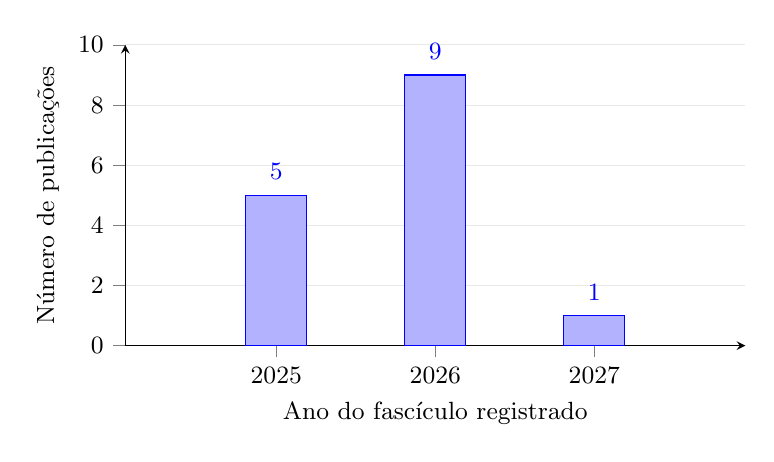
\begin{tikzpicture}
\begin{axis}[
  ybar, width=0.78\textwidth, height=5.4cm,
  ymin=0, ymax=10, xmin=0.5, xmax=3.5,
  ylabel={Número de publicações}, xlabel={Ano do fascículo registrado},
  xtick={1,2,3}, xticklabels={2025,2026,2027},
  ytick={0,2,4,6,8,10},
  axis lines=left, tick align=outside,
  ymajorgrids=true, grid style={gray!18},
  tick label style={font=\small}, label style={font=\small},
  nodes near coords, nodes near coords style={font=\small\bfseries, yshift=2pt},
  bar width=22pt, enlarge x limits=0.15,
  every axis plot/.append style={fill=teal!65!blue, draw=teal!65!blue!80!black}
]
\addplot coordinates {(1,5) (2,9) (3,1)};
\end{axis}
\end{tikzpicture}
